La technique est similaire au cas du triangle: nous allons obtenir une condition nécessaire, puis nous verrons que cette condition suffit via des arguments d'analyse. Cette dernière section nécessite plus de technicité.


% ----------------------- %


\begin{defi}
	Un \og \emph{$n$-gone} \fg\ désigne un polygone à $n$ côtés avec $n \geq 3$.
\end{defi}


\begin{defi}
	Un \og \emph{$n$-isogone} \fg\ désigne un $n$-gone dont tous les côtés sont de mesure égale.
\end{defi}


% ----------------------- %


\begin{fact} \label{conv-poly}
	Si un $n$-gone $\setproba{P}$ n'est pas convexe, alors on peut construire un $n$-gone convexe $\setproba{P}^{\,\prime}$ tel que 
	$\perim{\setproba{P}^{\,\prime}} = \perim{\setproba{P}}$ 
	et 
	$\area{\setproba{P}^{\,\prime}} > \area{\setproba{P}}$.
\end{fact}


\begin{proof}
	Ici, il ne faut pas être expéditif en indiquant que la preuve du fait \ref{quadri} se généralise sans aucun souci.
	En effet, avec $n > 4$, nous pouvons avoir plusieurs points de non-convexité, et les éliminer comme nous l'avons fait pour le quadrilatère n'est pas immédiat:
	dans la figure suivante, l'élimination des deux points de non convexité $G$ et $E$ de l'heptagone $ABCDEFG$ nous amène à un nouvel heptagone $ABCDE^{\,\prime}FG^{\,\prime}$ ayant lui aussi deux points de non-convexité $F$ et $D$!
	Donc, rien n'empêche, a priori, d'avoir une suite de constructions n'aboutissant jamais à un heptagone convexe
	de même périmètre que celui de $ABCDEFG$, et d'aire strictement supérieure à celle de $ABCDEFG$.%
	\footnote{
		L'auteur est convaincu que le procédé aboutira en un nombre fini d'étapes à un polygone convexe, mais il ne l'a pas démontré pour le moment.
	}

	\begin{center}
		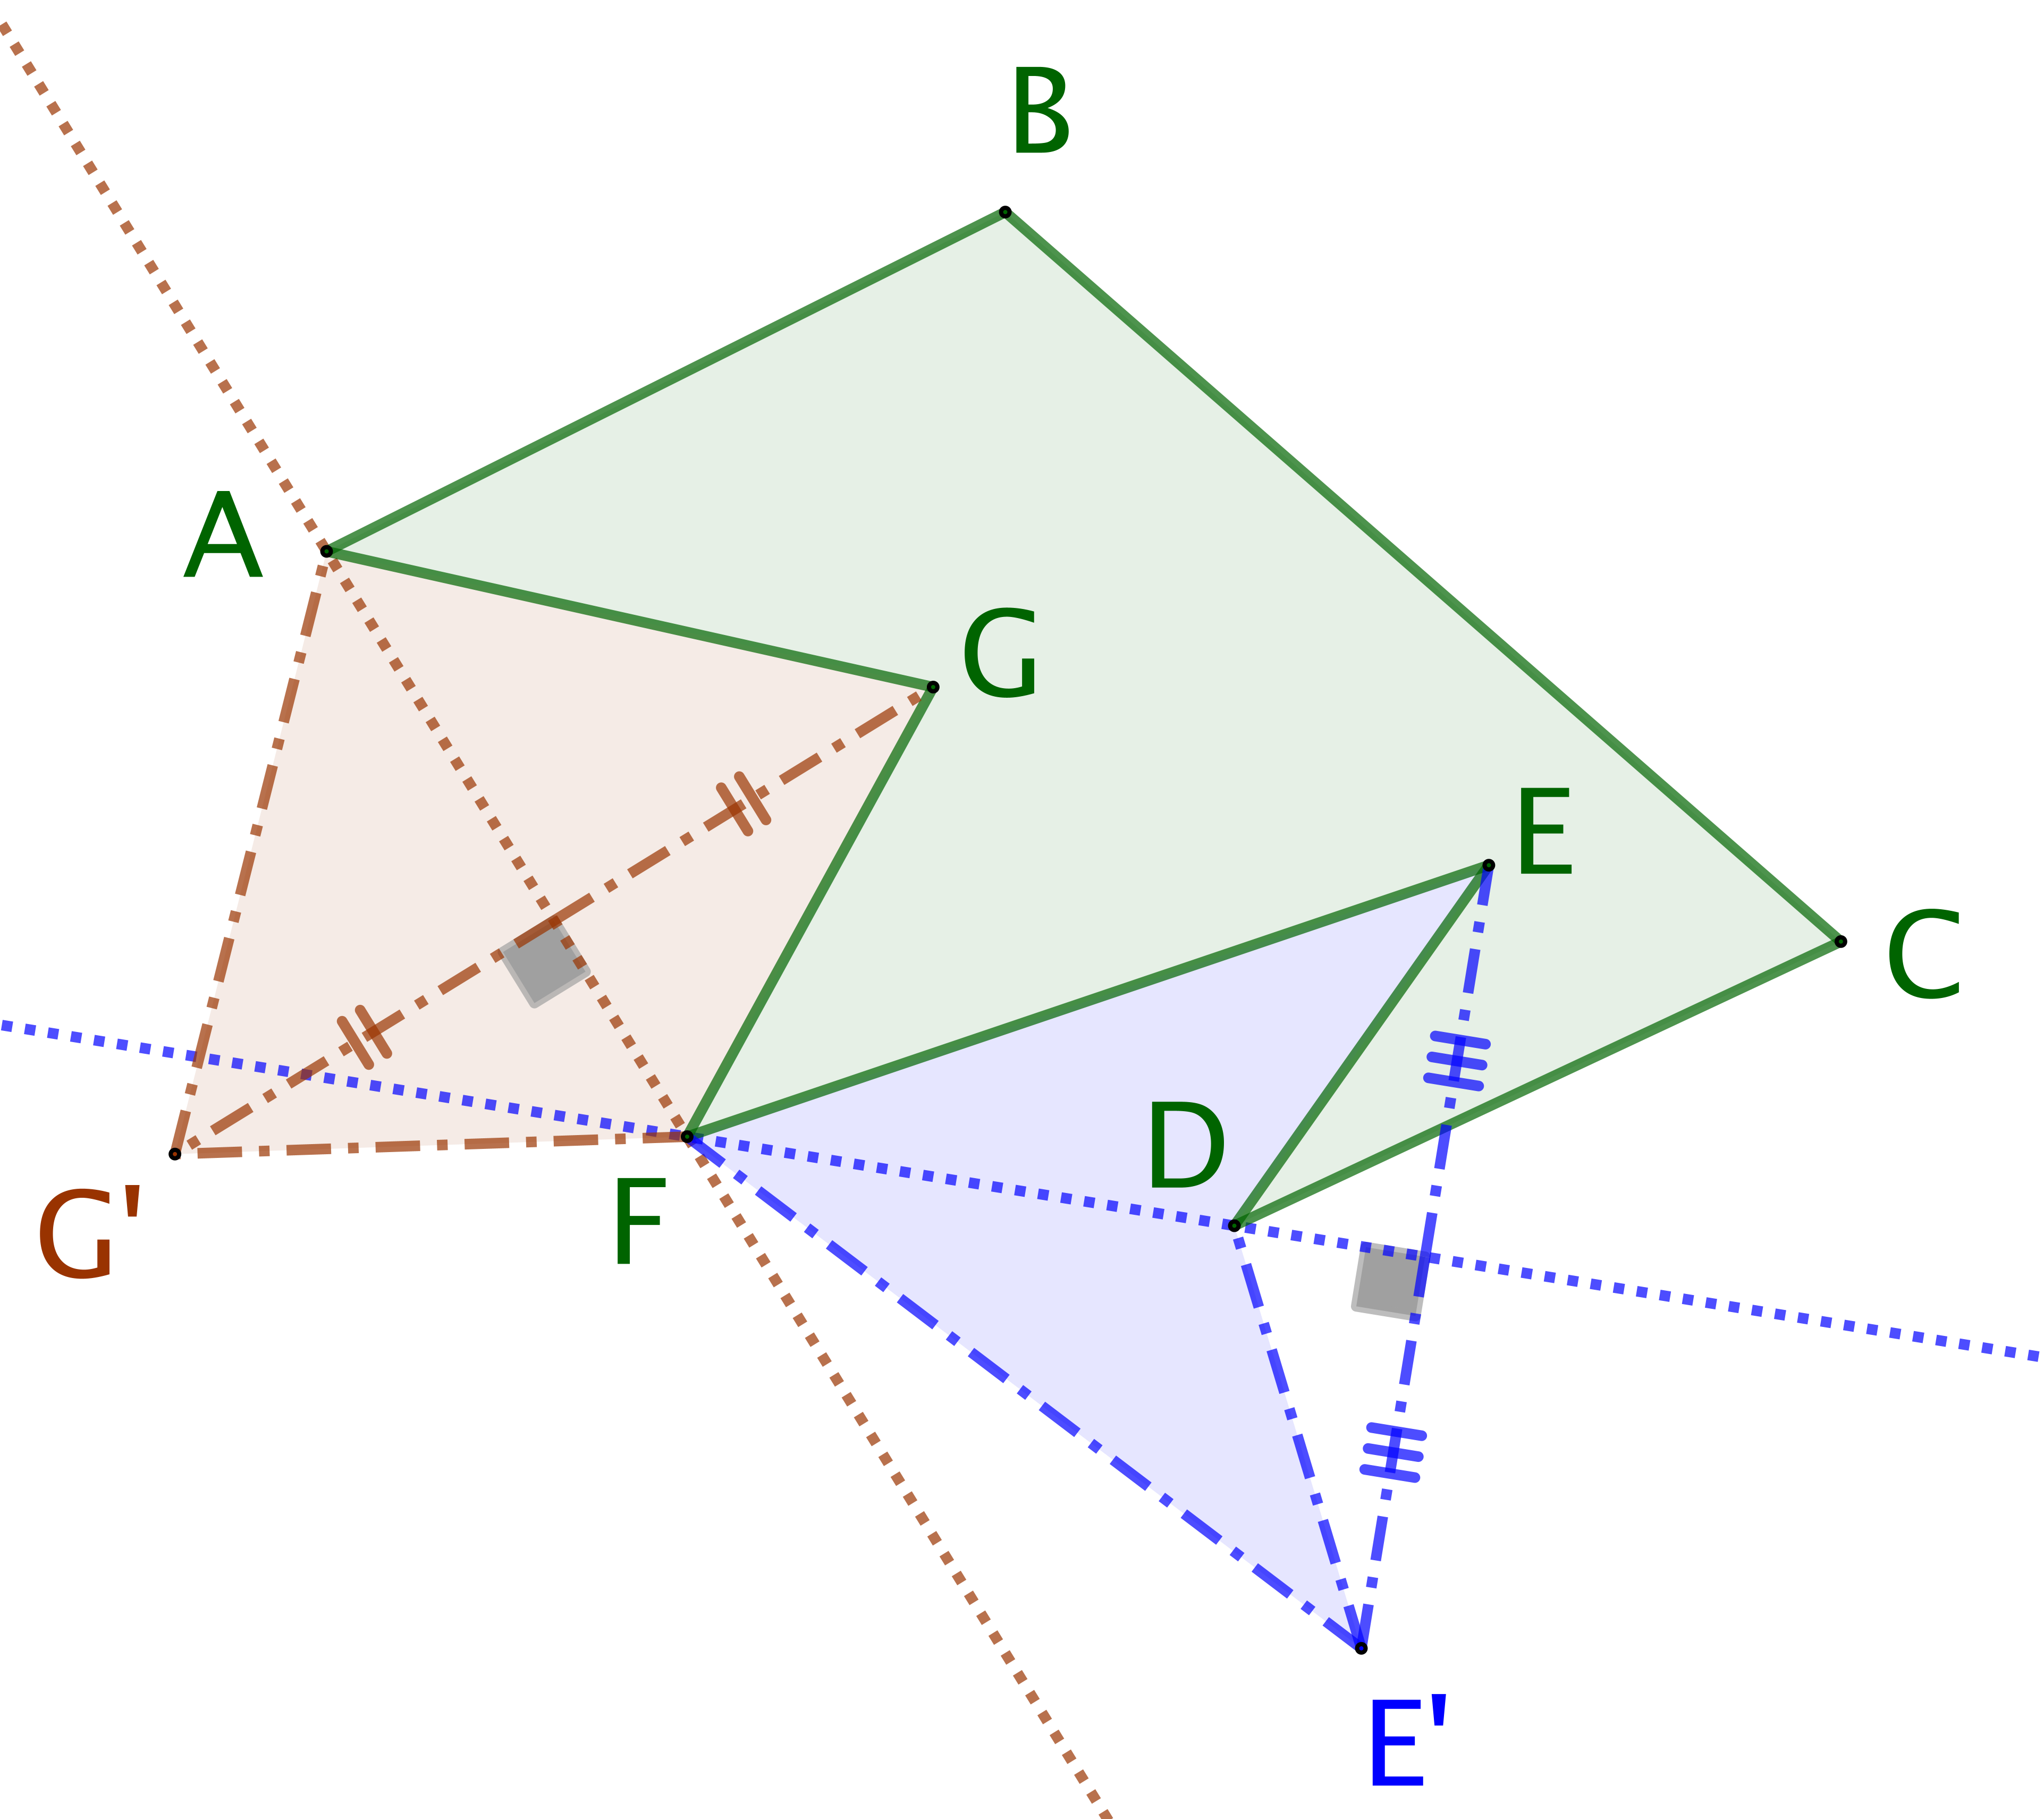
\includegraphics[scale=.4]{content/polygon/polygon-non-convex-trap.png}
	\end{center}
	

	Pire, on peut perdre des côtés lors de la construction comme dans l'exemple suivant où $C$, $D$ et $E^{\,\prime}$ sont alignés.

	\begin{center}
		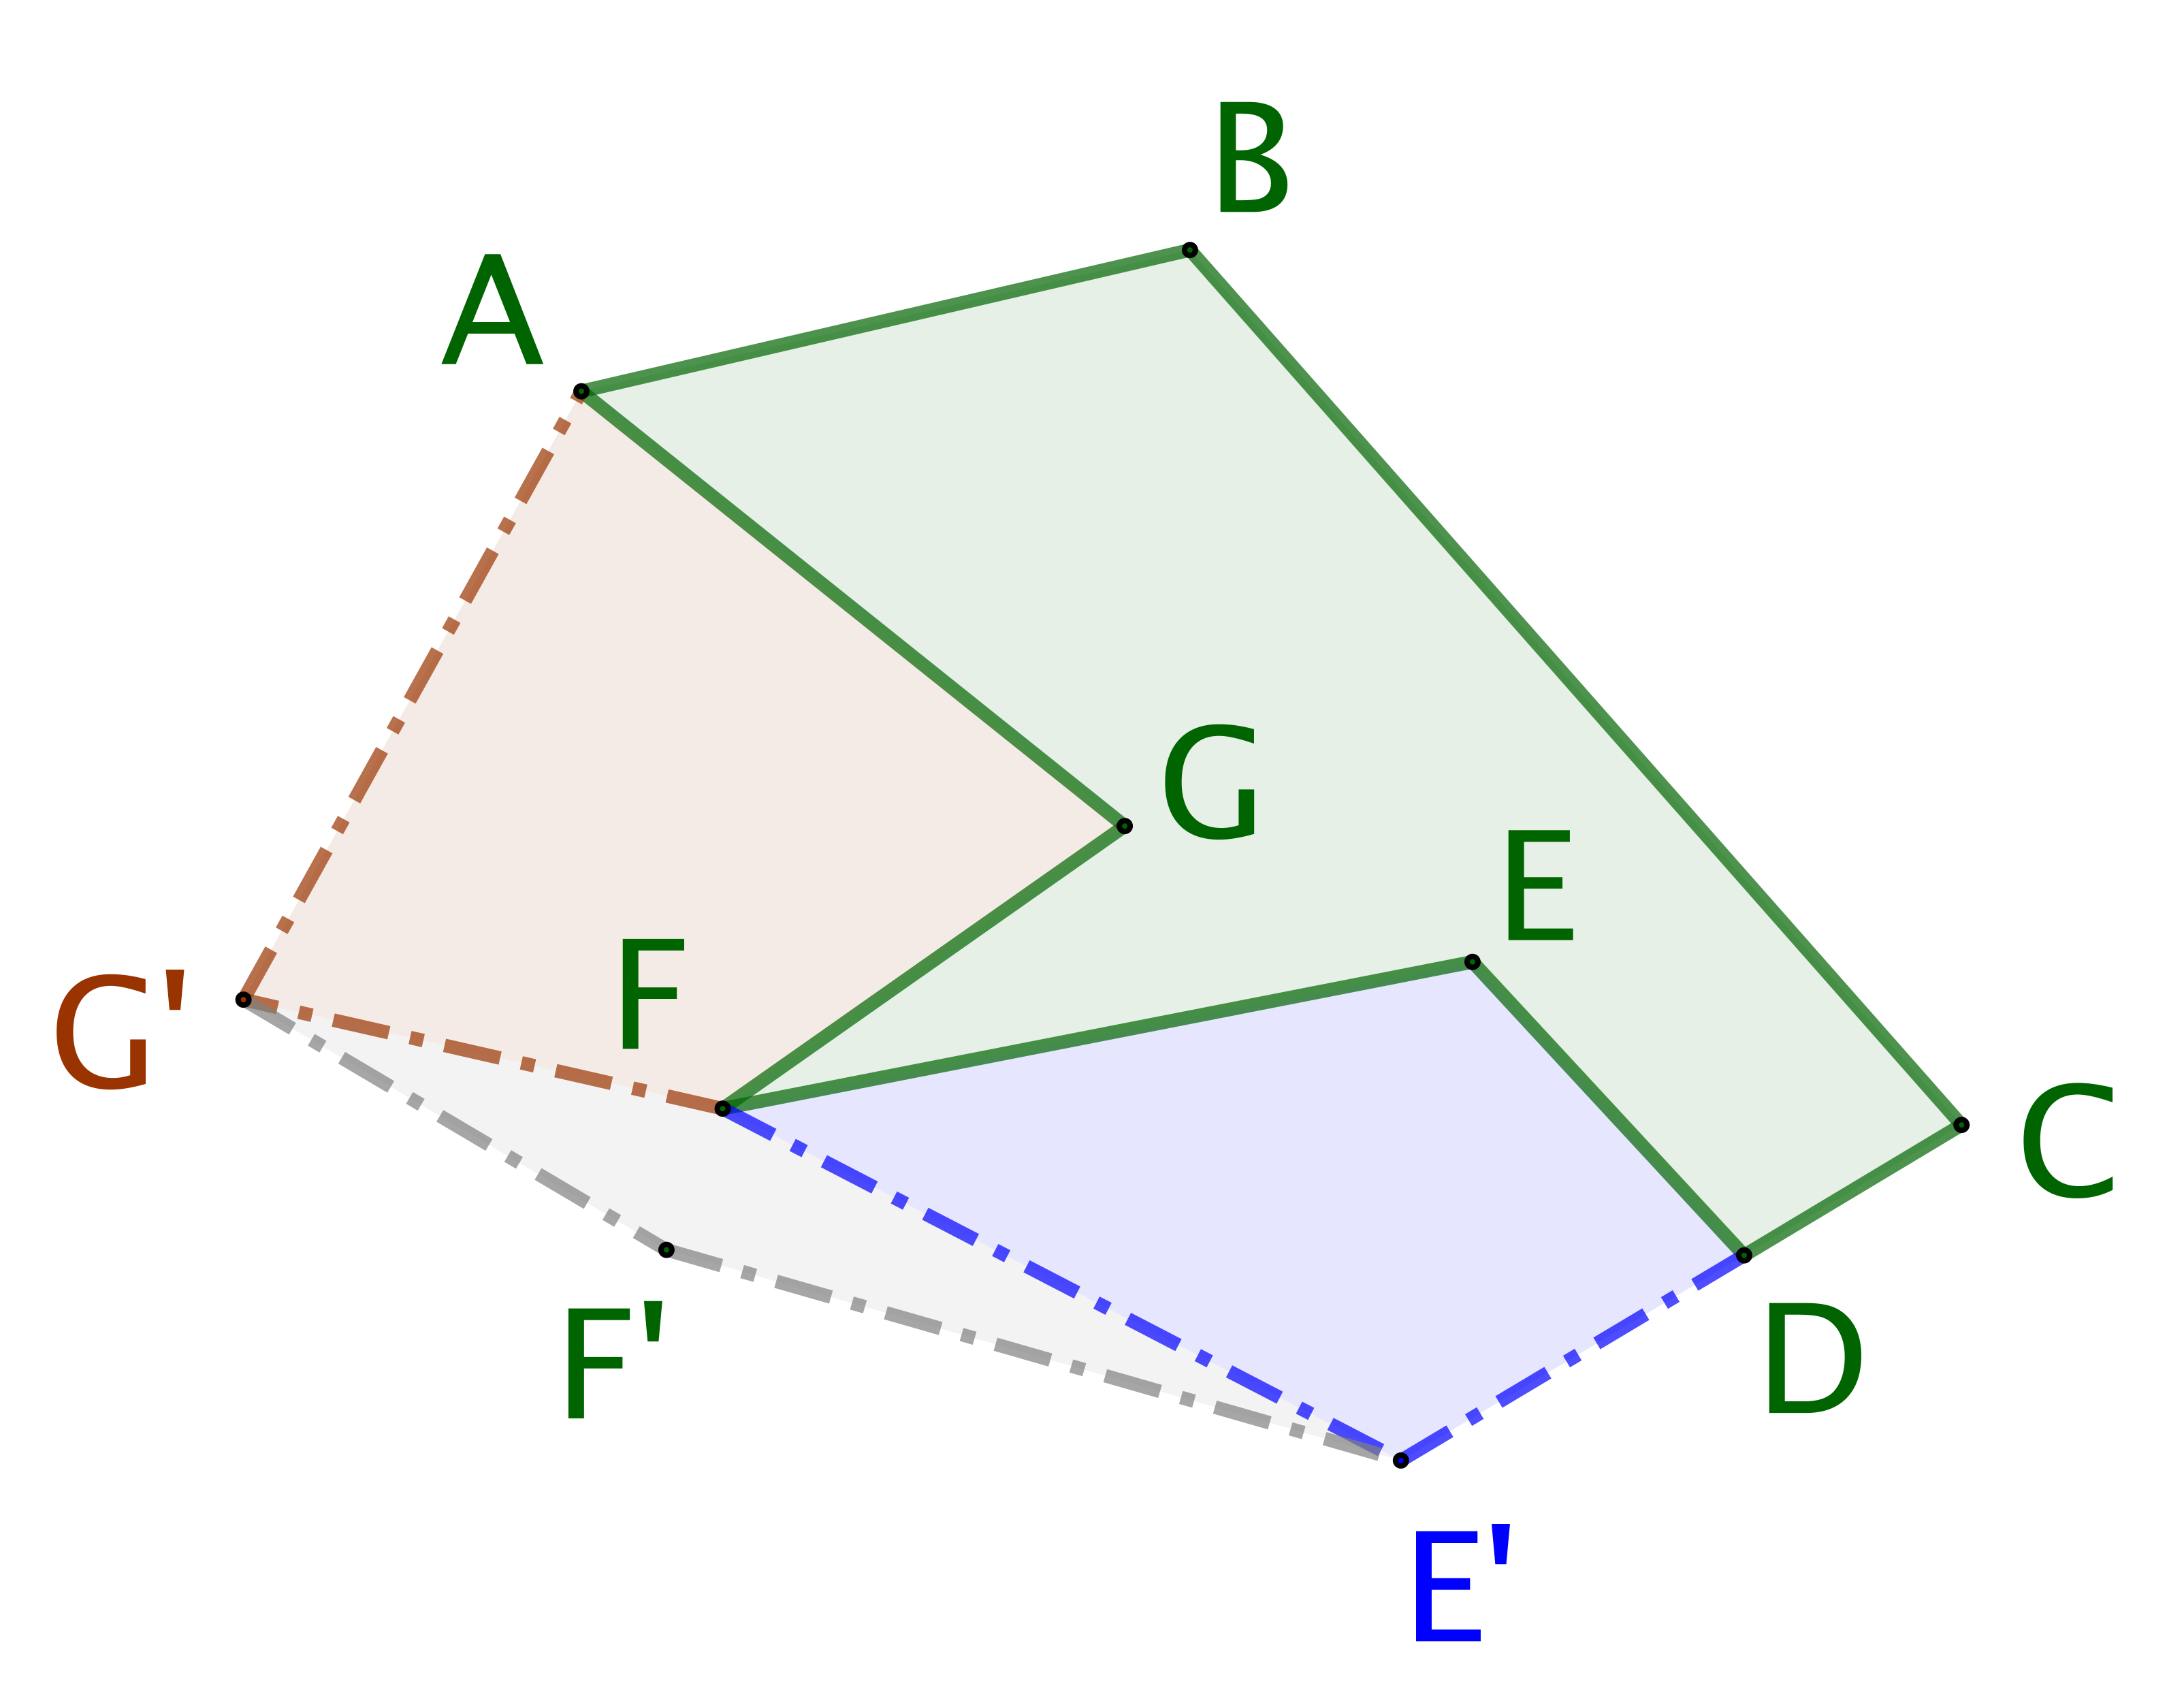
\includegraphics[scale=.4]{content/polygon/polygon-non-convex-bad.png}
	\end{center}


	Laissons de côté cette construction pour nous concentrer sur la classique enveloppe convexe%
	\footnote{
		C'est le plus petit polygone convexe \og \emph{contenant} \fg\ le $n$-gone considéré, où \og \emph{petit} \fg\ est relatif à l'inclusion.
	}
	du $n$-gone de départ.
	Par exemple, l'ennéagone $ABCDEFGHI$ non convexe ci-dessous admet le pentagone $ABDEG$ pour enveloppe convexe: le périmètre diminue et l'aire augmente, ce qui est utile, mais malheureusement le nombre de côtés change.
	
	\begin{center}
		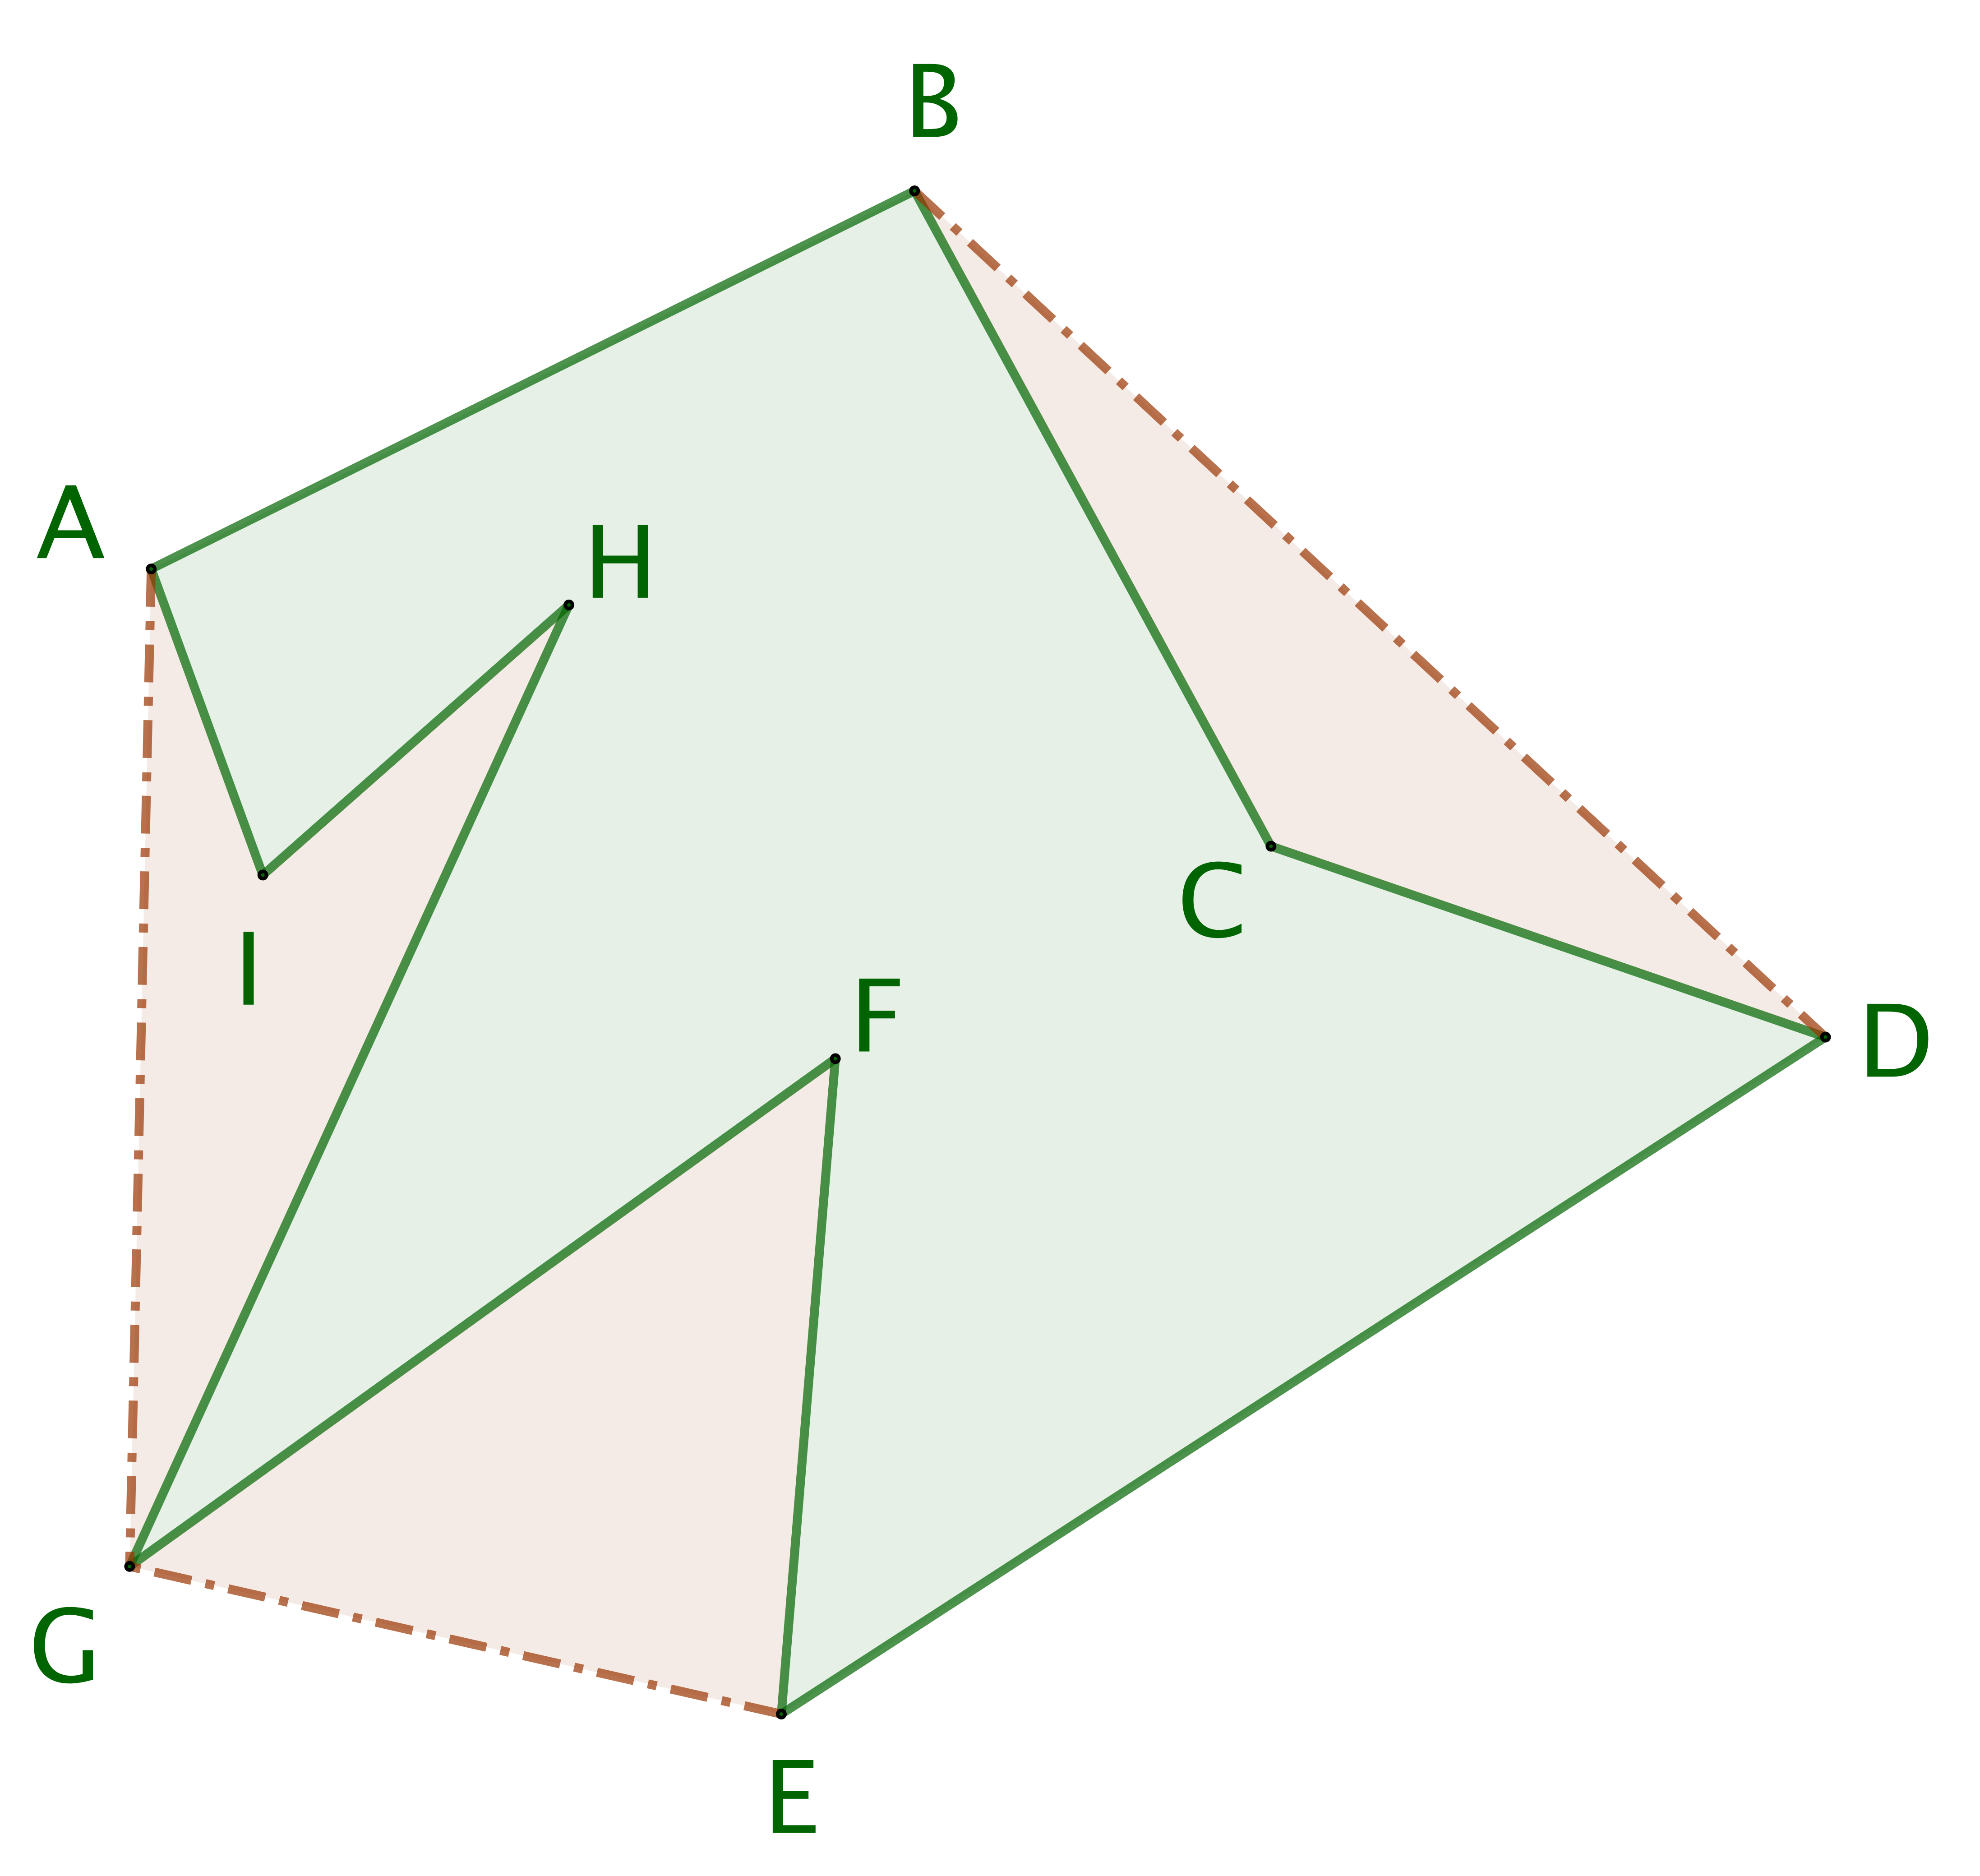
\includegraphics[scale=.4]{content/polygon/polygon-convex-hull.png}
	\end{center}

	Une idée simple, que nous allons formaliser rigoureusement juste après, consiste à ajouter les sommets manquants suffisamment prêts des côtés de l'enveloppe convexe afin de ne pas trop augmenter le périmètre pour le laisser inférieur, ou égal, à celui du $n$-gone non convexe initial. Le dessin suivant illustre cette idée.	
	
	\begin{center}
		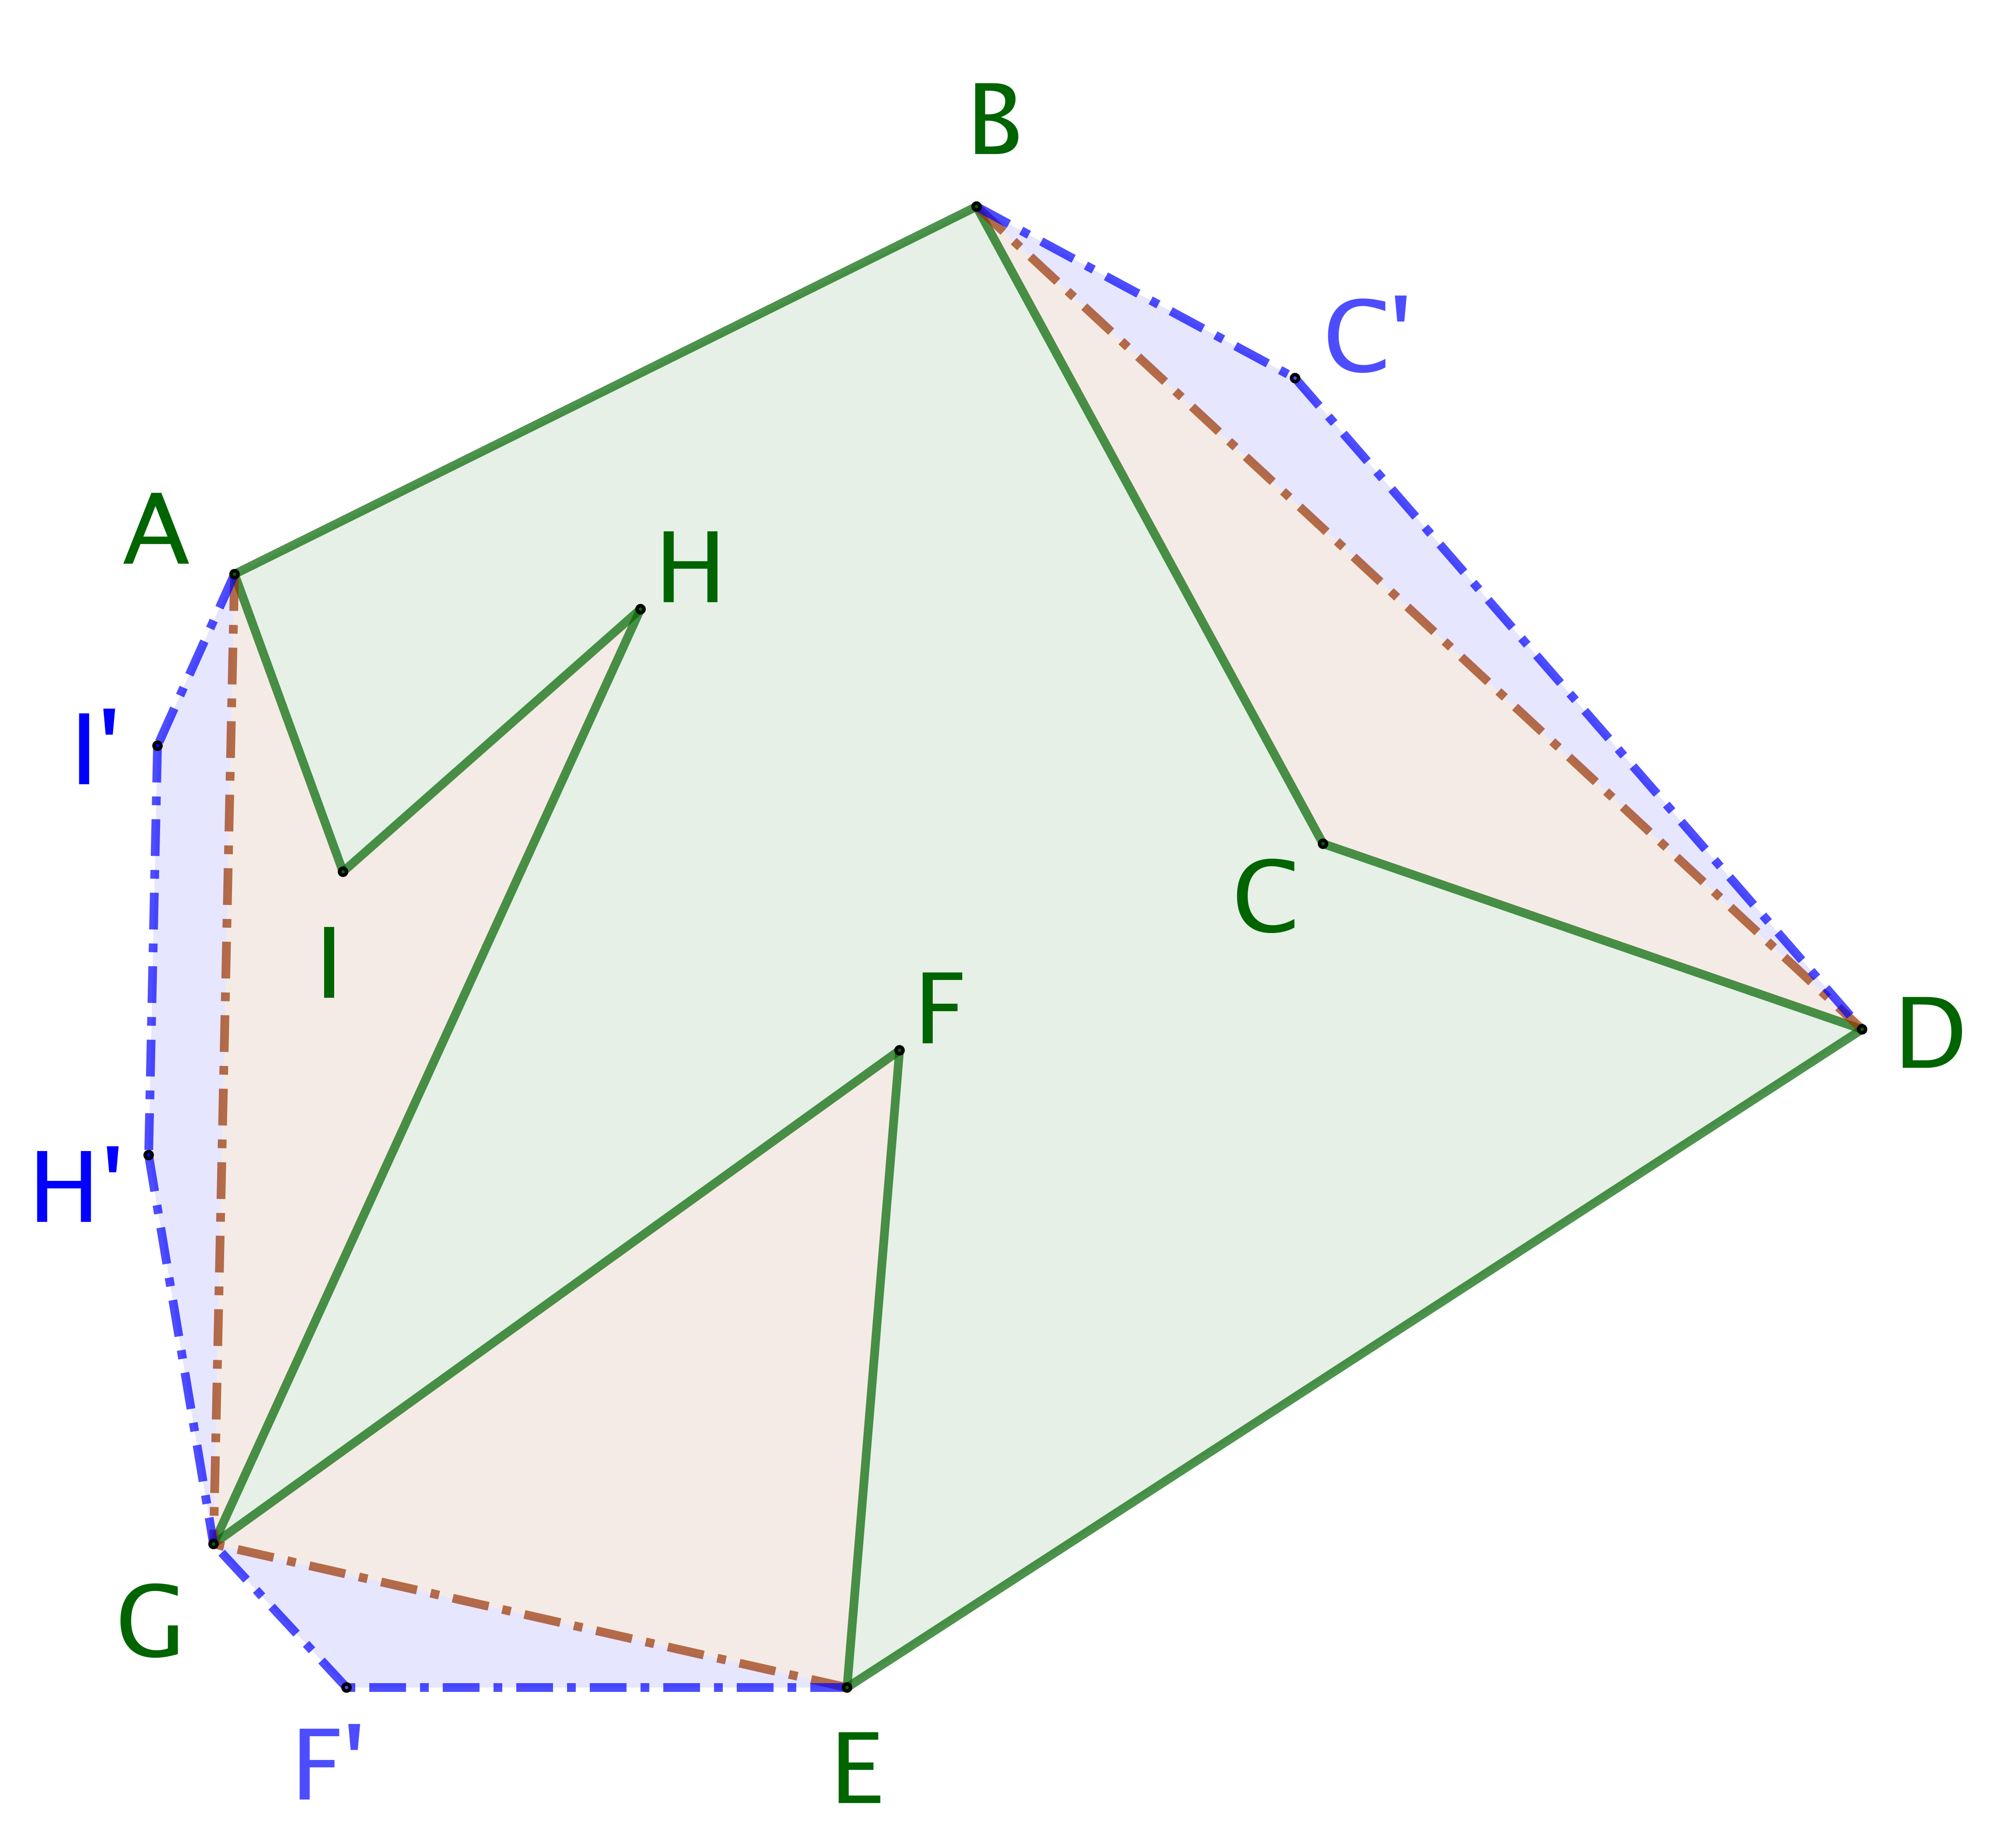
\includegraphics[scale=.4]{content/polygon/polygon-convex-hull-distortion.png}
	\end{center}

	Considérons donc un $n$-gone non convexe $\setproba{P}$, de périmètre $p$.
	%
	\begin{itemize}
		\item XXX

		\item XXX

		\item XXX

		\item XXX
	\end{itemize}
\end{proof}


% ----------------------- %


\begin{fact} \label{iso-poly}
	Si un $n$-gone convexe $\setproba{P}$ n'est pas un $n$-isogone, alors on peut construire un $n$-gone $\setproba{P}^{\,\prime}$ tel que 
	$\perim{\setproba{P}^{\,\prime}} = \perim{\setproba{P}}$ 
	et 
	$\area{\setproba{P}^{\,\prime}} > \area{\setproba{P}}$.
\end{fact}


\begin{proof}
	pas be soin d'isoccèle, on se place entre prolongement côté précédente et coté du traingle non isocèle et c'est réglé car périmtre dimnuer à aire constante !
	
	
	Considérons un $n$-gone convexe $\setproba{P}$, de périmètre $p$, qui n'est pas un $n$-isogone. 
	$\setproba{P}$ admet donc un triplet de sommets consécutifs $A$, $B$ et $C$ tels que $AB \neq AC$ (dans le cas contraire, on obtient de proche en proche un $n$-isogone).
	La construction vue dans la preuve du fait \ref{tri-one-side-fixed} permet de conclure sans effort ou presque.
	En effet,
	XXX
	si un sommet mangé, on fait de nouveau mini perturb pas supérieur à la pert de péimètre pour passer à iscoèle avant dilatation axiale
	
	non convexité pas gpenante car géré par le fait \ref{conv-poly}
	%
	\begin{itemize}
		\item XXX

		\item XXX

		\item XXX

		\item XXX
	\end{itemize}
\end{proof}


% ----------------------- %


\begin{fact} \label{almost-reg-poly}
	Si un $n$-isogone convexe $\setproba{P}$ possède deux angles de mesures différentes,
	alors il existe un $n$-gone $\setproba{P}^{\,\prime}$ tel que 
	$\degreg{\setproba{P}^{\,\prime}} > \degreg{\setproba{P}}$,
	$\perim{\setproba{P}^{\,\prime}} = \perim{\setproba{P}}$ 
	et 
	$\area{\setproba{P}^{\,\prime}} > \area{\setproba{P}}$.
\end{fact}


\begin{proof}
	wikipédia ok ? tjrs le pb du côté qui disparait !
	%
	\begin{itemize}
		\item XXX

		\item XXX

		\item XXX

		\item XXX
	\end{itemize}
\end{proof}


% ----------------------- %


\begin{fact}
	Soit $n \in \NN_{\geq3}$ un naturel fixé.
	Considérons tous les $n$-gones de périmètre fixé. Parmi tous ces $n$-gones, un seul est d'aire maximale, c'est le $n$-gone régulier.
\end{fact}


\begin{proof}
	on a cond necess vai les faits
	
	CS ca un max existe comme pour les triangles
	!!
	
	
	readc fausse
	refaire le chemind es restrictions !!!
	
	Tout a déjà été dit, car d'après les faits précédents, un $n$-gone $\setproba{P}$ non régulier ne peut pas maximiser son aire à périmètre fixé, et par conséquent seul le $n$-gone régulier maximise l'aire à périmètre fixé. Chapeau bas à vous, Géométrie et Analyse réunies...
\end{proof}
